% !TEX root = ../my-thesis.tex
%
\chapter{Introduction}
\label{sec:intro}

\cleanchapterquote{
	\textgreek{Δέδυκε μὲν ἀ σελάννα}\\
	\textsuperscript{The moon and the Pleiades}\\
	\textgreek{καὶ Πληΐαδες, μέσαι δέ}\\
	\textsuperscript{have set, it is}\\
	\textgreek{νύκτες, πάρα δ' ἔρχετ' ὤρα,}\\
	\textsuperscript{midnight, time is passing,}\\
	\textgreek{ἔγω δὲ μόνα κατεύδω.}\\
	\textsuperscript{but I sleep alone.}\\
}{Sappho, `The Midnight Poem'}{(c. 600 BC)}

% ---------------------------------------
\section{From seven sisters to a powerhouse of astronomy}
\label{sec:intro:intro}

In all of astronomy, few objects have retained relevance throughout the centuries as much as open clusters (OCs). Easily visible to the naked eye, the Pleiades has been observed since at least the dawn of civilisation CITEME, along with a handful of other OCs visible without a telescope. In the present day, the now thousands of known OCs are a key tool in modern astronomy for understanding stellar and galactic evolution.

Star clusters are formed when clouds of cold molecular gas collapse due to gravity, forming stars. Sometimes, when star formation occurs densely enough, these stars fall further into gravitationally bound clusters that can survive in the galactic disk for as long as $\sim 10^9$~years \citep{lada_embedded_2003,portegies_zwart_young_2010}. It is this property of the formation of OCs that makes them so useful: all stars in an OC will have the same age and initial composition, allowing parameters of the overall group of stars to be measured significantly more precisely than when studying stars in isolation. 

For instance, when a parameter such as the distance of member stars can simply be averaged over all member stars, then the precision of the mean distance of an OC (and hence the distance to all of its member stars) will be a factor $\sqrt{n}$ more precise than the distance to any individual star. Alternatively, when a property such as chemical composition is highly time consuming to derive, it can be derived for a fraction of stars in an OC and be applied to all stars in a cluster.

The ease of studying stellar astrophysics with OCs results in OCs having an extremely wide range of scientific use cases. For instance, OCs are used as testing grounds for stellar evolution models CITEME, as tracers of galactic structure \citep{cantat-gaudin_painting_2020,castro-ginard_milky_2021}, or even as calibrators of cepheid variable stars \citep{medina_revisited_2021}, which are an essential first rung on the cosmic distance ladder and are vital in the derivation of the cosmological parameters of the universe. It is somewhat of a cliché to describe OCs as `the laboratories of stellar evolution', but it really is true: OCs are a fantastic way to observe stars of a given age and composition across a broad range of masses, and to do so with orders of magnitude more precision than when studying isolated field stars.

The best part of the modern story of the OC's contribution to astrophysics comes with the \gaia\ satellite, however. In just five years since its first full data release \citep{brown_gaia_2018}, \gaia\ has revolutionised the study of our galaxy, including the study of OCs; with dozens of papers reporting thousands of new objects \citep[e.g.][]{liu_catalog_2019,castro-ginard_hunting_2019,castro-ginard_hunting_2020,castro-ginard_hunting_2022}, and a number of works deriving dramatically improved parameters and members for OCs in the Milky Way \citep[e.g.][]{cantat-gaudin_gaia_2018,tarricq_3d_2020}. Arguably, there has never been a better time to do science with OCs, owing to the incredible quantity and quality of data that \gaia\ has provided.

There is, however, a catch. Even though the Milky Way is estimated to contain as many as $10^5$ OCs \citep{dias_new_2002}, there are still only a few thousand currently known in the literature -- representing a small fraction of the total number of OCs in our galaxy. It has been shown that the census of OCs is incomplete within even 1~kpc from the Sun \citep[e.g.][]{castro-ginard_new_2018}, and the extent of the remaining incompleteness is unknown. Worse still, it has been shown that many of the OCs catalogued previously in the literature may not exist \citep{cantat-gaudin_clusters_2020,piatti_catching_2023}, with it being largely unknown which OCs are or are not real. The many fantastic uses of OCs in other areas of astronomy are contingent on a reliable, accurate, and complete census of OCs; and the many current caveats with the census of OCs limit the science potential of these fantastic objects in a time when we have more available data with which to study them than ever before.

In this thesis, I will present solutions to a number of the current issues with the OC census in the era of \gaia, using a range of data analysis and parameter inference techniques. I will then use these techniques to create the largest census of OCs to date and derive a range of parameters for these OCs. With this thesis, I also hope to present methods that could continue to be used to maximise the quality of the OC census for the coming decade of \gaia\ data releases -- as well as for whatever instruments supercede \gaia\ in the future.

Before launching into the chapters detailing my work over the past three and a half years, it is worth first conducting an overview of the science behind OCs in the introduction to this thesis. In Sect.~\ref{sec:intro:history}, I will discuss the history of OC observations up to before the release of \gaia\ DR2 in 2018, as well as briefly discussing the techniques and results from pre-\gaia\ observations. Section~\ref{sec:intro:gaia} will then discuss the stunning data of \gaia\ and how it has already thoroughly revolutionised our understanding of OCs in just a handful of years. Finally, Sect.~\ref{sec:intro:theory} will briefly discuss some key pieces of theory surrounding the structure, dynamics, and lifetime of OCs, providing a good background on our theoretical knowledge of OCs that will assist with the reading of this thesis.

The nomenclature and definition of star clusters varies throughout the literature. Hence, in the next section, I will quickly discuss a definition of OCs that I will adopt throughout the rest of this work.


% ---------------------------------------
\section{The definition of an open cluster}
\label{sec:intro:definition}

\begin{figure}[tb]
	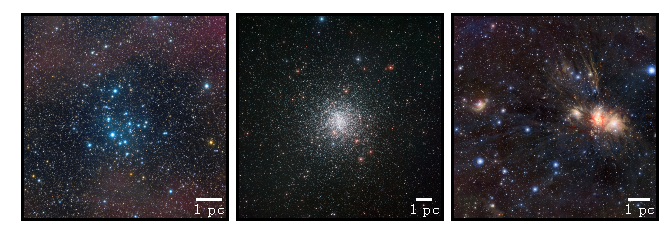
\includegraphics[width=\textwidth]{fig/c1/oc_gc_mg_comparison.pdf}
	\caption[A visual comparison between the three main types of star cluster found in the Milky Way.]{A visual comparison between the three main types of star cluster found in the Milky Way. \emph{Left:} the open cluster NGC~2547. \emph{Middle:} the globular cluster M~4. \emph{Right:} the moving group/OB association Monoceros~R2. All images contain a scale in the bottom right showing a length of 1~pc at the distance of each cluster. NGC~2547 is a sparser OC that has a clear core of young blue stars at its center, about $\sim 1$~pc across. On the other hand, despite being only slightly larger, M~4 clearly contains significantly more stars. The stars in M~4 are older, with the cluster having a whiter or redder appearance. On the other hand, Monoceros~R2 is simply a group of young blue stars, with no discernible core. \emph{Credit, left to right:} ESO / J. Pérez; ESO; ESO / J. Emerson / VISTA. }
	\label{fig:intro:definition:comparison}
\end{figure}

There are many different types of star cluster in the universe. This thesis will exclusively discuss clusters observed in the Milky Way, and will primarily discuss open clusters (OCs), although I will also touch on globular clusters (GCs) and moving groups (MGs). Avoiding confusion when talking about star clusters is important; hence, I differentiate between these three types of cluster approximately as follows, matching the definition in \cite{portegies_zwart_young_2010}.

OCs are gravitationally bound clusters with a typical age of around 100~Myr, although some are older than 1~Gyr and some are as young as 0.1~Myr. OCs have masses of typically no greater than $10^4$~\MSun and may be made up of a few dozen to a few thousand stars, with a typical minimum being ten stars. OCs are remants of recent star formation and are hence predominantly located in the galactic disk where the star formation rate is highest. Most OCs have a size of around 3 to 10~pc. Other than some exceptions, OCs contain a single population of stars. 

GCs are much older and more massive gravitationally bound clusters, with ages typically greater than 10~Gyr and masses typically greater than $10^5$~\MSun. The largest GCs can contain a million stars or more. GCs have a typical size around 10 to 20~pc. GCs tend to reside in the galactic bulge or in the galactic halo. Many GCs contain multiple populations of stars. Almost all OCs have masses significantly lower than the typical present day mass of GCs, although observations of a handful of young massive clusters in the Milky Way such as Westerlund~1 (sometimes also referred to as `super star clusters') as well as observations of galaxies with more active star formation suggest that the highest mass star clusters will be long-lived and will evolve into GCs. However, this is not the case for almost all OCs that I will study in this thesis, as the only young massive clusters in the Milky Way are generally distant, heavily reddened, and outside of the reach of the visual-band observations of the \gaia\ telescope.

On the other hand, MGs are of a similar mass and number count to OCs, except they are not gravitationally bound. Due to this, they disperse much more quickly, and hence often have much younger ages. MGs have the widest definition, and encompass any group of stars that are comoving and coeval, but are specifically \emph{not} gravitationally bound. Some MGs are also referred to as `OB associations' in the literature, due to them often containing a number of young, high mass O and B stars. 

\begin{table}[tb]
	\begin{tabularx}{\textwidth}{l | X | X | X | X}
		\hline\hline
		Type & Bound? & Age & Mass & Location \\
		\hline
		Open cluster (OC)   & Weakly & $\lesssim 1$ Gyr & $\lesssim 10^4$ \MSun & Disk \\
		Globular cluster (GC)   & Strongly & $\gtrsim 10$ Gyr & $\gtrsim 10^5$ \MSun & Halo/Bulge \\
		Moving group (MG)   & No & $\lesssim 50$ Myr & $\lesssim 10^3$ \MSun & Disk\\
		\hline
	\end{tabularx}
	\caption{Approximate definitions for the three types of star cluster that will be discussed in this thesis.\label{tab:intro:definition:definition}}
\end{table}

These definitions are summarised in Table~\ref{tab:intro:definition:definition} and compared visually in Fig.~\ref{fig:intro:definition:comparison}.





% ---------------------------------------
\section{The history and techniques of open cluster observations}
\label{sec:intro:history}

\blindtext

% Plot of the pleiades
\begin{figure}[tb]
	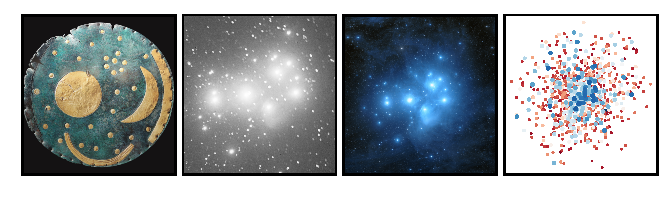
\includegraphics[width=\textwidth]{fig/c1/pleiades.pdf}
	\caption[The Pleiades as depicted throughout history.]{The Pleiades, as depicted throughout history and showing the clear improvements in astronomical data gathering over time. \emph{Left:} the Nebra Sky Disc, depicting the Pleiades with its seven naked-eye visible stars in the upper center. The disc was discovered in 1999 in northern Germany and is dated to between 1800-1600 BC. \emph{Middle left:} the Pleiades, as imaged in 1909 with Wolf's Doppelastrograph at the Landessternwarte Heidelberg-Königstuhl. \emph{Middle right:} the Pleiades, as imaged by Hubble. \emph{Right:} the $\sim$1000 member stars for the Pleiades extracted from \gaia\ DR2 data and isolated from field stars by \cite{cantat-gaudin_characterising_2018}. Each star is represented by a point scaled by its magnitude and coloured according to its $BP-RP$ colour. \emph{Image credits:} Frank Vincentz; Heidelberg Digitized Astronomical Plates; Davide De Martin / NASA/ESA Hubble.}
	\label{fig:intro:history:pleiades}
\end{figure}

% Plot of catalogues of OCs
\begin{figure}[tb]
	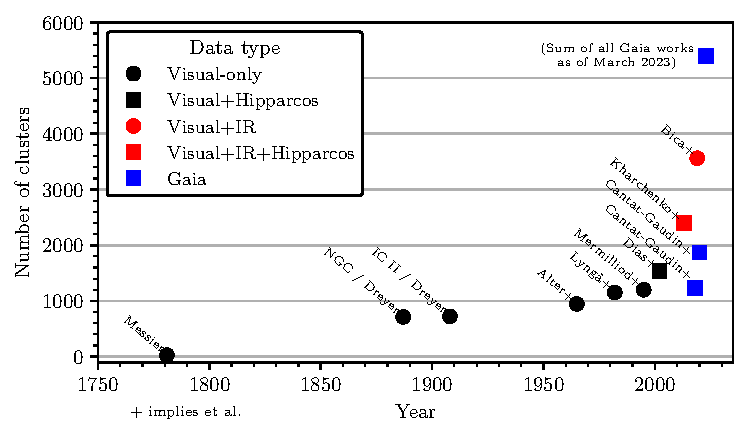
\includegraphics[width=\textwidth]{fig/c1/catalogues.pdf}
	\caption{TODO}
	\label{fig:intro::history:catalogues}
\end{figure}


% Plot of reported OCs
\begin{figure}[tb]
	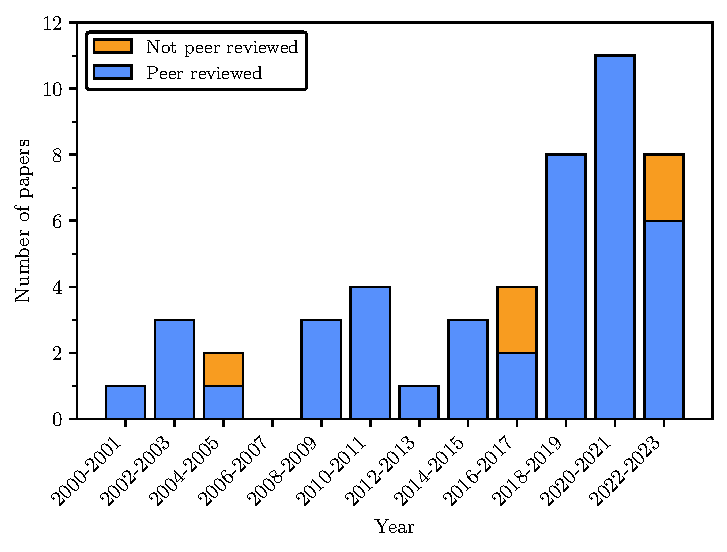
\includegraphics[width=\textwidth]{fig/c1/papers.pdf}
	\caption{TODO}
	\label{fig:intro:history:papers}
\end{figure}


% ---------------------------------------
\section{The \gaia\ revolution in open cluster science}
\label{sec:intro:gaia}


% ---------------------------------------
\section{Some theoretical background into star clusters}
\label{sec:intro:theory}


% ---------------------------------------
\section{Thesis structure}
\label{sec:intro:structure}

\textbf{Chapter \ref{sec:intro}} \\[0.2em]
\blindtext

\textbf{Chapter \ref{sec:intro}} \\[0.2em]
\blindtext

\textbf{Chapter \ref{sec:intro}} \\[0.2em]
\blindtext

\textbf{Chapter \ref{sec:intro}} \\[0.2em]
\blindtext

\textbf{Chapter \ref{sec:intro}} \\[0.2em]
\blindtext
